\documentclass[tekniskrapport/tech.tex]{subfiles}

%Sammanfattningen bör innehålla:
%
%   -En beskrivning av de mest framträdande egenskaperna hos det totala
%   systemet och de olika delsystemen.
%
%   -Ett blockschema som beskriver konstruktionens uppdelning i olika delar.
%
%   -En beskrivning av vilka sensorer som ska användas och hur de ska placeras.
%
%   -En beskrivning av vilka ställdon (motor etc,) som ska användas och hur
%   de ska användas och hur de ska placeras.

\begin{document}

\section{Översikt}
Under den här punkten förklaras designen av systemet översiktligt.

\subsection{Framträdande egenskaper}
Produkten består av tre moduler: Kommunikation-, sensor- och styrmodul, vilka implementeras på ett virkort. Produkten, som ansluts till en fjärklient via WLAN, har två avståndsmätare och en kamera till hjälp när information om produktens omgivning samlas in. Vardera mikrokontroller klockas med en kristalloscillator.

\begin{figure}[h]
    \centering
    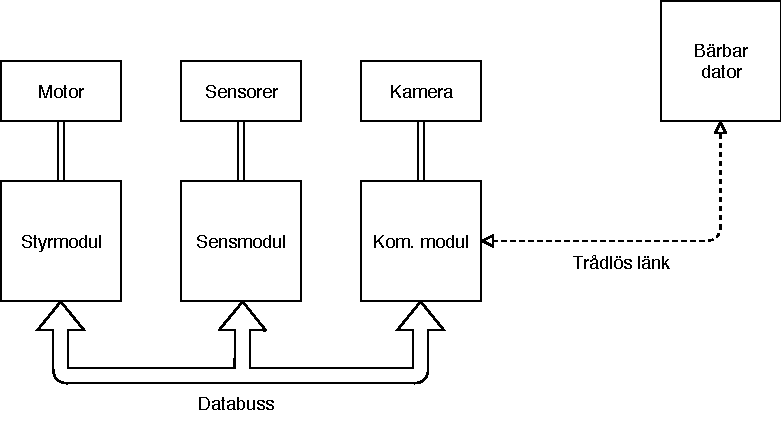
\includegraphics[width=0.4\linewidth]{\figures/blockskiss.pdf}
    \caption{Övergripande bild över systemet och dess moduler. SPI-buss används}
    \label{fig:overview}
\end{figure}

\noindent
Kommunikationsmodulen, vilken består av en Raspberry Pi, fungerar som en central
kommun\-ikations- och beslutsenhet som ansvarar för att ta beslut om taxins
beteende samt hantera kommunikationen mellan modulerna. Styrmodulen, vilken består av
en motor och en mikrokontroller, står för drift samt reglering av taxins
hastighet och svängradie. Sensormodulen består av en mikrokontroller samt
avståndsmätare och halleffektsensorer monterade på bilens hjul.

\subsection{Sensorer}
Kameran har satts upp på bilens framsida vid en specifik höjd och lutad neråt enligt bildbehandlings behov. Avståndsmätaren, vilken hjälper vid upptäckandet av hinder genom att mäta avståndet till det, har också placerats på bilens framsida längre ner kameras position.
Som tidigare sagts, innehåller bilen två avståndsmätare; den tidigare nämnda på framsidan och en till, vilken har fäst på bilens bakre högersida och som kan användas för att avgöra när ett hinder har passerats vid omkörning. Odometern som används till att mäta kördistans är redan färdigmonterad på chassit.

\subsection{Ställdon}
Hjulen, motorn och ställdonen är redan färdigmonterade. Motorn används
för att få bilen att åka framåt och bakåt medan en servo används för att svänga.

\end{document}
